\section{Basic Idea}
\subsection{I/O activity-based allocation}
\subsubsection{Fallacy: LBA-based lifetime prediction}
+ in-place update workload will be added \\ \\
Many existing data separation techniques such as~\cite{AutoStream, HotCold} 
estimate the data lifetime based on the update frequency of LBAs.  
For example, \textsf{\small AutoStream}~\cite{AutoStream} assumes that, if
some LBAs are frequently rewritten by applications, those LBAs hold hot data.
This LBA-based lifetime prediction 
approach, however, does not work well with recent data-intensive 
applications where a majority of
new data are written in an append-only manner.  

In order to illustrate a mismatch between an LBA-based predictor and 
append-only workloads, we analyzed the write pattern of 
RocksDB~\cite{RocksDB}, which is a
popular key-value store based on the LSM-tree algorithm~\cite{LSM}.
Fig.~\ref{fig:lba_lifetime}(a) shows how LBAs may be related 
to data lifetimes\footnote{The lifetime of data is defined 
by the logical time which is the number of writes to the device 
between when the data is first written 
and when the data is invalidated by an overwrite or a TRIM command.}
in RocksDB~\cite{RocksDB}.  
As shown in Fig.~\ref{fig:lba_lifetime}(a), 
there exists no strong correlation between the LBAs and lifetimes in RocksDB.  
This scatter plot is in sharp contrast with one for update workloads 
where a few distinct LBA regions have short lifetimes while others 
have very long lifetimes.

\begin{figure}[t]
	\centering
	\hfill
	%\vspace{-9pt}
	%\captionsetup[subfigure]{margin={0cm,1cm}}
	\subfloat[Lifetime patterns over LBAs]{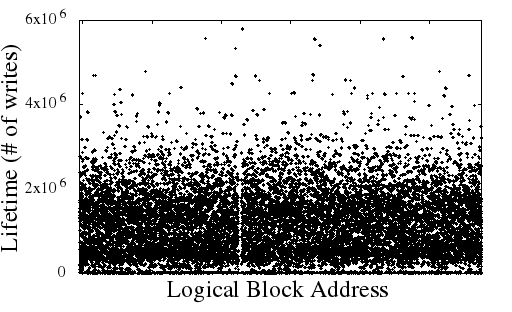
\includegraphics[width=0.215\textwidth]{figure/lba_lifetime2}}  % data from 0/03031641
	\hspace{10pt}
	\subfloat[Lifetime patterns over time]{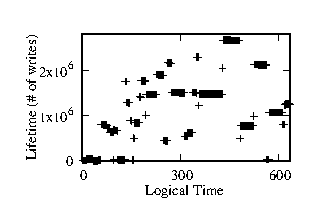
\includegraphics[width=0.21\textwidth]{figure/lifetime_in_chunk}}
	%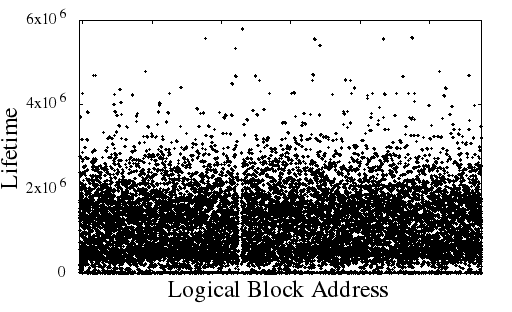
\includegraphics[width=0.9\linewidth]{figure/lba_lifetime} 
	%\vspace{-3pt}
	\caption{Lifetime distributions over addresses and times.} %shane part
	\label{fig:lba_lifetime}
	%\vspace{-20pt}
\end{figure}


We also analyzed 
if the lifetimes of LBAs change under some predictable patterns over time 
although the overall lifetime distribution shows large variances.
Fig.~\ref{fig:lba_lifetime}(b) shows a scatter plot of data lifetimes over the logical time 
for a specific 1-MB chunk with 256 pages. 
As shown in Fig.~\ref{fig:lba_lifetime}(b), 
for the given chuck, data lifetimes vary in a random fashion
(although some temporal locality is observed).
\begin{comment}
Over the logical time, the lifetime of data written to the chunk 
varies in an unpredictable fashion.  
For example, at the logical time 10, the lifetime was 1 but it increases about 
2.6 million around the logical time 450 
followed by a rapid drop around the logical time 600. 
\end{comment}
Our illustration using RocksDB strongly suggests that under append-only
workloads, LBAs are not useful in deciding data lifetimes.

\subsubsection{Program context as a lifetime predictor}
In developing \textsf{\small PCStream}, our key insight was that in most applications,
(regardless of their I/O workload characteristics)
a few dominant I/O activities exist
and each dominant I/O activity   
represents the application's important I/O context (e.g., for logging or for flushing). 
Furthermore, most dominant I/O activities tend to have distinct data lifetime patterns.
In order to distinguish data by their lifetimes, therefore, 
it is important to effectively distinguish dominant I/O activities from each other.  
For example, in update workloads, 
LBAs alone were effective in separating dominant I/O activities.  


\begin{comment}
In developing PCStream, we started from a simple question: 
how can we extract I/O context from an application? 
For example, in RocksDB, logging, flushing and compaction can be regarded
as different I/O contexts.
RocksDB appends write-ahead logs to storage to ensure data
persistence.  Those logs have short lifetimes because they are quickly deleted
after original data are persistently stored.
The flush module (which materializes the content of a memtable in
DRAM, called an L0 table, to an L1 table in the storage) generates data
with relatively short lifetimes. This is because an L1 table will be flushed to
an L2 table and be removed in the near future. Conversely, a compaction module
writes long-lived data that are unlikely to be removed for a long time.

The above observation implies that, if we are able to know the detailed
behaviors of append-only applications, data with different lifetimes can be
isolated in separate streams in an SSD. As mentioned before, a common
solution~\cite{MultiStream} to realizing this is manually modify an application
code so that each module assigns a unique stream ID to data it generates.
However, owing to considerable implementation efforts required to modify
individual applications, this approach is not widely used in practice.
\end{comment}

In this paper, we argue that a program context is an efficient  general-purpose
indicator for separating dominant I/O activities regardless of the type of I/O
workloads.  Since a PC represents an execution path of an application which
invokes write-related system functions such as {\tt write()} and {\tt writev()}
in the Linux kernel,  we represent the PC by summing program counter values of
all the functions along the execution path which leads to a write system call.
In RocksDB, for example, dominant I/O activities include logging, flushing and
compaction.  Since they are invoked through different function-call paths, we
can easily identify dominant I/O activities of RocksDB using PCs.  For example,
Fig.~\ref{fig:getpc}(a) shows an execution path for flushing in RocksDB.  The
sum of program counter values of \texttt{Run()}, \texttt{WriteLevel0Table()},
and \texttt{BuildTable()} is used to represent the PC for the flushing
activity.  Note that using the program context to distinguish data lifetimes is
not new.  For example, Ha {\it et al.} proposed a data separation technique
based on the program context~\cite{PCHa}.   However, their work was neither
designed for append-only workloads nor for modern multi-streamed SSDs.

\begin{figure}[t]
\centering
\hfill
%\vspace{-10pt}
	\subfloat[Logging (PC)]{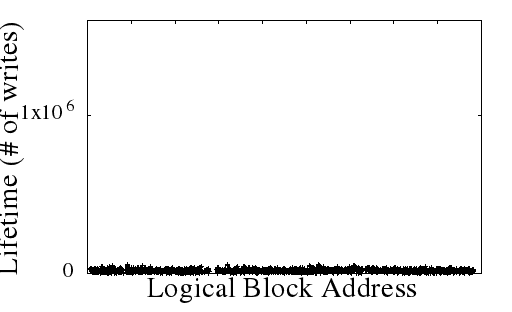
\includegraphics[width=0.2\textwidth]{figure/type_1}} % data from 4/03031953 
	\hspace{2pt}
	\subfloat[Logging (manual)]{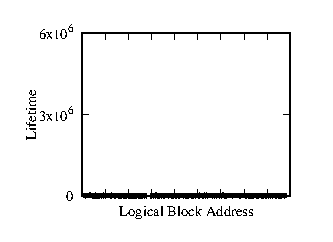
\includegraphics[width=0.2\textwidth]{figure/pcID_2}}
\hfill
\vspace{7pt}
	\subfloat[Flushing (PC)] {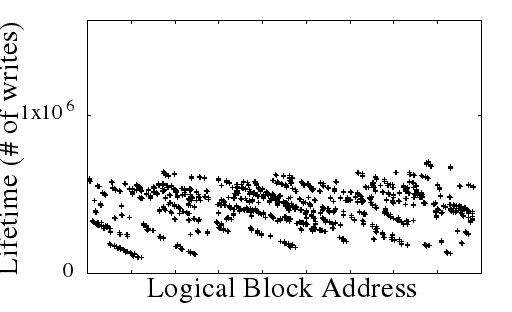
\includegraphics[width=0.2\textwidth]{figure/type_3}}
	\hspace{2pt}
	\subfloat[Flushing (manual)]{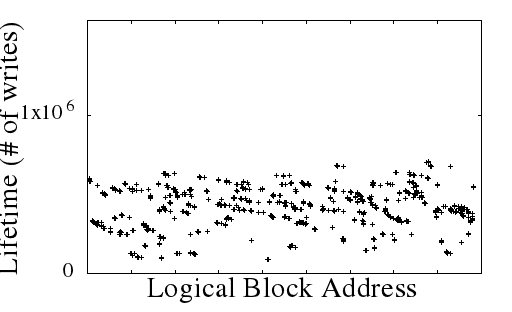
\includegraphics[width=0.2\textwidth]{figure/pcID_3}}
%\vspace{-7pt}
\caption{Data lifetime distributions of different PCs.} 
\label{fig:types_and_PCs}
%\vspace{-20pt}
\end{figure}


In order to validate our hypothesis that PCs can be useful for predicting
lifetimes by distinguishing dominant I/O activities, we conducted experiments
using RocksDB, comparing the accuracy of identifying dominant I/O activities
using two different methods.  First, we manually identified dominant I/O
activities by inspecting the source code. Second, we automatically decided
dominant I/O activities by extracting PCs for write-related system functions.
Fig.~\ref{fig:types_and_PCs} illustrates two dominant I/O activities matched
between two methods.   As shown in Fig.~\ref{fig:types_and_PCs}(a)
and~\ref{fig:types_and_PCs}(b), the logging activity of RocksDB is correctly
identified by two methods.  Furthermore, from the logging-activity PC, we can
clearly observe that data written from the PC are short-lived. Similarly,
from Fig.~\ref{fig:types_and_PCs}(c) and~\ref{fig:types_and_PCs}(d), we observe
that data written from the flushing-activity PC behave in a different fashion.
For example, data from the flushing-activity PC remain valid a lot longer than
those from the logging-activity PC.


\subsection{Two-phase stream management}
\subsubsection{Limited number of streams}

It is advantageous to support a large number of streams in order to manage data with different lifetime characteristics as distinct streams.
Therefore, the multi-stream specification defines up to 65536 streams [].
However, the number of streams actually supported by an SSD that implements the specification is limited to 4 to 16[].
This is a limitation that occurs because there are restrictions on the resource required to implement multi-stream. It can be divided into memory, power, and overprovision resource.

First, memory resource may limit the number of multi-stream.
The controller that runs the SSD provides various memories such as TCM, SRAM, and DRAM. 
To optimize the performance, frequently referenced data structures should be located in fast memory.
The size of the data structure associated with a multi-stream is proportional to the number of streams supported and is directly related to performance, so it must be located in fast memory.
However, because of limited memory sizes, such as TCM or SRAM,
 there is a limit to the number of streams that can be supported with good performance.

Second, power resource may limit the number of multi-stream.
SSDs that support multi-stream are used in data centers or storage servers. SSDs use tantalum or electrolytic capacitors as backup power to guarantee data integrity even under sudden power off conditions.
Buffered data that is used to effectively utilize the parallelism of flash ensures reliable write to flash by using backup power during power off detection.
Since the buffered data is managed per stream, its size increases in proportion to the number of streams.
This also limits the number of streams that can be supported because SSDs use limited backup power at the limited PCB size.

Lastly, overprovision resource may limit the number of multi-stream.
As the number of multi-stream support increases, the active point increases. 
For each active point, it is necessary to allocate separate flash blocks.
 As the number of streams increases, it causes a decrease in overprovision area of SSD.
However, since the overprovisioning area of the SSD is limited, if the number of streams becomes too large, there may be a problem of increase of WAF due to overprovision reduction. 
In the case of streams over the number of overprovisioned blocks, flash block allocation  is not possible.
 

\subsubsection{I/O activity with large lifetime variance}
For most PCs, their lifetime distributions tend to have small variances.  
However, we observed that a few outlier PCs which have large lifetime variations. 
For example, when multiple I/O contexts are covered by the same write system function, 
the corresponding PC may represent several I/O contexts whose data lifetimes are quite different.   
Such a case occurs, for example, 
in the compaction module of RocksDB.
RocksDB maintains
several levels, L1, ..., L$n$, in the persistent storage, except for L0 (or a
memtable) stored in DRAM.  Once one level, say L2, becomes full, all the data
in L2 is compacted to a lower level, i.e., L3.  It involves moving data from L2
to L3, along with the deletion of the old data in L2.  In the
LSM tree~\cite{LSM}, a higher level is smaller than a lower level 
(i.e., the size of (L2) $<$ the size of (L3)). 
Thus, data stored in a higher level is invalidated more frequently than those kept
in lower levels, thereby having shorter lifetimes.

%Once the L1 becomes full,
%\textit{all} the data kept in the L1 are moved to the L2 by the compaction
%module.  The same operation is applied to the other levels (i.e., L3, ...,
%L$n-1$).  The compaction involves reading and writing data from a higher level
%(e.g., L1) to a lower level (e.g., L2).  The data in a higher level (e.g., L1)
%is then removed.  

%While the program context can be used as a useful indicator that determines the
%lifetime of data, we also observe that the same PC could generate data 
%with diverged lifetimes. One of the representative examples is the compaction
%module of RocksDB. RocksDB maintains several levels, L1, ..., L$n$, in the
%persistent storage, except for L0 (or a memtable) stored in DRAM.  Data flushed
%from the memtable are first written to the L1.  Once the L1 becomes full,
%\textit{all} the data kept in the L1 are moved to the L2 by the compaction
%module.  The same operation is applied to the other levels (i.e., L3, ...,
%L$n-1$).  The compaction involves reading and writing data from a higher level
%(e.g., L1) to a lower level (e.g., L2).  The data in a higher level (e.g., L1)
%is then removed.  In the LSM-tree, a higher level is smaller than a lower
%level. Thus, data stored in a higher level is invalidated sooner than data kept
%in lower levels, thereby having much shorter lifetimes.

Unfortunately, in the current RocksDB implementation, the compaction step is supported 
by the same execution path (i.e., the same PC) regardless of the level.
Therefore, the PC for the compaction activity cannot effectively separate data with 
short lifetimes from one with long lifetimes.
Fig.~\ref{fig:compaction}(a) shows 
the lifetime distribution collected from the compaction-activity PC.  
Since this distribution includes lifetimes of data written from all the levels, 
its variance is large.  
When we manually separate the single compaction step into several per-level compaction steps, 
as shown in Figs. 5(b) and 5(c), the lifetime distributions of per-level compaction steps 
show smaller variances.   
In particular, L2 and L3 show distinct lifetime distributions from that of L4.
Data from L2 and L3 are likely to have shorter lifetimes, while L4 has generally
long-lived data as shown in Fig. 5(d).

\begin{figure}[!t]
\centering
%\vspace{-7pt}
\hfill
\subfloat[compaction: all levels]{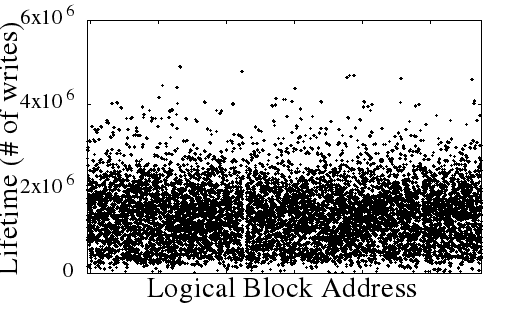
\includegraphics[width=0.19\textwidth]{figure/pc_3}}
	\hspace{2pt}
\subfloat[compaction: L2]{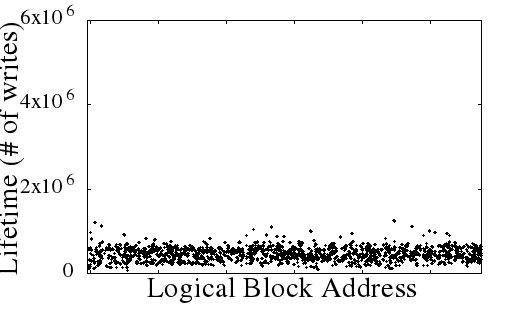
\includegraphics[width=0.19\textwidth]{figure/type_4}}  % data from 4/03040047
\hfill
\vspace{-1pt}
\subfloat[compaction: L3]{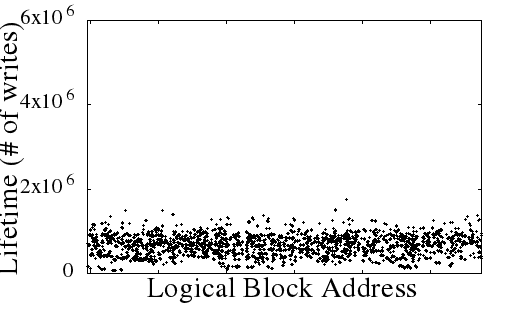
\includegraphics[width=0.19\textwidth]{figure/type_5}}
	\hspace{2pt}
\subfloat[compaction: L4]{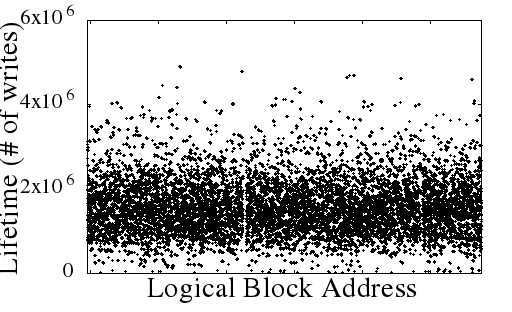
\includegraphics[width=0.19\textwidth]{figure/type_6}}
%\vspace{-10pt}
%\caption{The lifetime distribution of the compaction activity.} 
\caption{Lifetime distributions of the compaction activity at different levels.} %shane part
\label{fig:compaction}
%\vspace{-20pt}
\end{figure}

\subsubsection{Separating long-lived data during GC}
Since it is difficult to separate data with different lifetimes within the same PC 
(as in the compaction-activity PC), we devised a two-phase method that decides SSD 
streams in two levels: the main stream ID in a host level and the substream ID in an SSD level.
Conceptually, long-lived data in the main stream are moved to its substream to 
separate from (future) short-lived data of the main stream.
Although moving data to the substream may increase WAF,
the overhead can be hidden if we restrict the substream move during GC only.
Since long-lived data (i.e., valid pages) in a victim block are moved to a free block during GC, 
they can be moved to the substream by changing the target block.
For instance, \textsf{\small PCStream} assigns the compaction-activity PC {\it pID} to a
main stream {\it sID} for the first phase.
To separate the long-lived data of {\it pID} (e.g., L4 data) 
from future short-lived data of {\it pID} (e.g., L1 data), 
valid pages of the {\it sID} are assigned to its substream for the second phase during GC.


